\begin{figure}[htbp]
			\centering
			\begin{tikzpicture}[
				scale=0.95,
				>=latex,
				trave/.style={line width=2pt},
				carico/.style={black, line width=0.8pt},
				forza/.style={black, line width=1pt},
				diagN/.style={black, line width=0.8pt},
				hatch/.style={gray!50, line width=0.3pt},
				quota/.style={black, line width=0.4pt},
				]
				
				% ── Parametri dei vincoli (convenzione C06/C07) ──
				\def\tw{0.15}    \def\thR{0.28}   \def\rn{0.06}
				\def\rw{0.05}    \def\bw{0.09}    \def\gw{0.22}
				\def\hh{0.10}
				
				% ── Geometria ──
				\def\Lell{4}                 % lunghezza trave ℓ
				\def\cC{8/3}                 % posizione di C (= 2ℓ/3)
				\def\yq{-0.80}               % y della quota
				\def\ylab{\yq-0.7}           % y delle etichette di pannello (allineate)
				
				% =========================================================
				% PANNELLO (a) — Schema strutturale
				% =========================================================
				\begin{scope}[xshift=0cm]
					
					% Trave
					\draw[trave] (0,0) -- (\Lell,0);
					
					% Cerniera in A
					\draw[thick] (0,0) -- (-\tw,-\thR) -- (\tw,-\thR) -- cycle;
					\draw[thick] (-\gw,-\thR) -- (\gw,-\thR);
					\foreach \x in {-0.16,-0.08,0,0.08,0.16}
					\draw[thin] (\x,-\thR) -- ++(-0.07,-\hh);
					
					% Carrello trasversale in B
					\draw[thick] (\Lell,0) -- (\Lell-\tw,-\thR) -- (\Lell+\tw,-\thR) -- cycle;
					\draw[thick] (\Lell-\bw,-\thR-\rw-0.01) circle (\rw);
					\draw[thick] (\Lell+\bw,-\thR-\rw-0.01) circle (\rw);
					\draw[thick] (\Lell-\gw,-\thR-2*\rw-0.04) -- (\Lell+\gw,-\thR-2*\rw-0.04);
					\foreach \x in {-0.16,-0.08,0,0.08,0.16}
					\draw[thin] (\Lell+\x,-\thR-2*\rw-0.04) -- ++(-0.07,-\hh);
					
					% Anellini
					\draw[thick, fill=white] (0,0) circle (\rn);
					\draw[thick, fill=white] (\Lell,0) circle (\rn);
					
					% Etichette A, B, C
					\node[above left=-2pt,  font=\small] at (0,0)       {$A$};
					\node[above right=-2pt, font=\small] at (\Lell,0)   {$B$};
					\node[below,  font=\small] at (\cC,-0.04) {$C$};
					
					% ── Carico triangolare q(z) = q̄ z/ℓ ──
					\def\hbase{0.22}    \def\hmax{1.20}    % h(0)=0, h(ℓ)=hmax-hbase
					
					% (1) frecce longitudinali, in linea con la base del riquadro
					\pgfmathsetmacro{\yfre}{\hbase+0.10}
					\foreach \t in {0.05, 0.20, 0.35, 0.50, 0.65, 0.80,0.95} {
						\pgfmathsetmacro{\px}{\Lell*\t}
						\draw[->, carico] (\px, \yfre) -- (\px + 0.30, \yfre);
					}
					
					% (2) triangolo soprastante con campitura verticale di altezza variabile
					\foreach \x in {0.25, 0.50, ..., 3.75} {
						\pgfmathsetmacro{\htop}{\hbase + (\hmax-\hbase)*\x/\Lell}
						\draw[hatch] (\x, \hbase) -- (\x, \htop);
					}
					% bordo del triangolo: base + ipotenusa + lato verticale destro
					\draw[carico, line width=0.6pt]
					(0, \hbase) -- (\Lell, \hbase) -- (\Lell, \hmax) -- cycle;
					
					% (3) etichetta del carico, sopra il vertice di destra
					\node[right, font=\small] at (\Lell, \hmax-0.1) {$\bar{q}$};
					
					% ── Forza concentrata Z(C) = q̄ℓ/4 in C ──
					\def\Lf{0.55}
					\pgfmathsetmacro{\yC}{0.10}     % freccia leggermente sopra l'asse
					% tacca verticale che marca il punto di applicazione C
					\draw[forza] (\cC, \yC-0.08) -- (\cC, \yC+0.08);
					% freccia da C verso destra
					\draw[->, forza] (\cC, \yC) -- (\cC + \Lf, \yC);
					% etichetta sopra la freccia
					\node[below, font=\small] at (\cC + 0.8*\Lf, \yC-0.04)
					{$\tfrac{\bar{q}\ell}{4}$};
					
					% ── Quota 2ℓ/3 sotto la trave ──
					\draw[<->, quota] (0,\yq) -- (\cC,\yq);
					\draw[quota] (0,\yq+0.07) -- (0,\yq-0.07);
					\draw[quota] (\cC,\yq+0.07) -- (\cC,\yq-0.07);
					\node[above, font=\small] at (0.5*\cC, \yq-0.04) {$\tfrac{2}{3}\ell$};
					
					% Etichetta pannello
					\node[font=\small] at (0.5*\Lell, \ylab+0.2) {(a)};
					
				\end{scope}
				
				% =========================================================
				% PANNELLO (b) — Diagramma di N(z)
				% =========================================================
				\begin{scope}[xshift=6cm]
					
					% Trave (clone)
					\draw[trave] (0,0) -- (\Lell,0);
					
					% Vincoli (clone esatto dal pannello a)
					\draw[thick] (0,0) -- (-\tw,-\thR) -- (\tw,-\thR) -- cycle;
					\draw[thick] (-\gw,-\thR) -- (\gw,-\thR);
					\foreach \x in {-0.16,-0.08,0,0.08,0.16}
					\draw[thin] (\x,-\thR) -- ++(-0.07,-\hh);
					\draw[thick] (\Lell,0) -- (\Lell-\tw,-\thR) -- (\Lell+\tw,-\thR) -- cycle;
					\draw[thick] (\Lell-\bw,-\thR-\rw-0.01) circle (\rw);
					\draw[thick] (\Lell+\bw,-\thR-\rw-0.01) circle (\rw);
					\draw[thick] (\Lell-\gw,-\thR-2*\rw-0.04) -- (\Lell+\gw,-\thR-2*\rw-0.04);
					\foreach \x in {-0.16,-0.08,0,0.08,0.16}
					\draw[thin] (\Lell+\x,-\thR-2*\rw-0.04) -- ++(-0.07,-\hh);
					\draw[thick, fill=white] (0,0) circle (\rn);
					\draw[thick, fill=white] (\Lell,0) circle (\rn);
					\node[left,  font=\small] at (0,-0.04)     {$A$};
					\node[right, font=\small] at (\Lell,-0.04) {$B$};
					\node[below,  font=\small] at (\cC,-0.04) {$C$};
					\draw[forza] (\cC, -0.10) -- (\cC, 0.10);
					
					% ── Diagramma N(z) ──
					% Scala: 1 q̄ℓ = \sN unità di figura
					\def\sN{1.70}
					% Valori notevoli (in unità "q̄ℓ"):
					%   N(0)       = 3/4
					%   N(2ℓ/3⁻)   = 19/36
					%   N(2ℓ/3⁺)   = 5/18 = 10/36
					%   N(ℓ)       = 0
					\pgfmathsetmacro{\NA}{(3/4)*\sN}        % 3/4 q̄ℓ in A
					\pgfmathsetmacro{\NCm}{(19/36)*\sN}     % 19/36 q̄ℓ in C⁻
					\pgfmathsetmacro{\NCp}{(10/36)*\sN}     % 10/36 q̄ℓ in C⁺
					
					% Hatching sotto l'arco parabolico
					% Tratto AC: N(z) = (3/4 − z²/(2ℓ²)) q̄ℓ
					\foreach \x in {0.10, 0.30, ..., 2.55} {
						\pgfmathsetmacro{\h}{(3/4 - (\x*\x)/(2*\Lell*\Lell))*\sN}
						\draw[hatch] (\x, 0) -- (\x, \h);
					}
					% Tratto CB: N(z) = (ℓ²−z²)/(2ℓ²) q̄ℓ = (1/2)(1−(z/ℓ)²) q̄ℓ
					\foreach \x in {2.75, 2.95, ..., 3.85} {
						\pgfmathsetmacro{\h}{(1/2)*(1 - (\x*\x)/(\Lell*\Lell))*\sN}
						\draw[hatch] (\x, 0) -- (\x, \h);
					}
					
					% Bordo: assi verticali + parabole + raccordi
					% verticale in A
					\draw[diagN] (0, 0) -- (0, \NA);
					% parabola AC con \draw plot
					\draw[diagN, smooth, samples=20, domain=0:\cC]
					plot (\x, {(3/4 - (\x*\x)/(2*\Lell*\Lell))*\sN});
					% verticale del salto in C
					\draw[diagN] (\cC, \NCm) -- (\cC, \NCp);
					% parabola CB
					\draw[diagN, smooth, samples=20, domain=\cC:\Lell]
					plot (\x, {(1/2)*(1 - (\x*\x)/(\Lell*\Lell))*\sN});
					% (in B il diagramma chiude naturalmente a y=0, niente verticale)
					
					% Segno "+" (trazione) cerchiato, al centro dell'area
					\node[circle, draw, fill=white, thick,
					minimum size=10pt, inner sep=0pt, font=\large]
					at (0.5*\cC, 0.35*\sN) {$+$};
					
					% Etichette dei valori notevoli
					\node[below left,  font=\small] at (0,    \NA)  {$\tfrac{3}{4}\bar{q}\ell$};
					\node[right, font=\small] at (\cC-0.1,  \NCm) {$\tfrac{19}{36}\bar{q}\ell$};
					\node[left,  font=\small] at (\cC+0.1,  \NCp-0.18) {$\tfrac{5}{18}\bar{q}\ell$};
					
					% Etichetta pannello
					\node[font=\small] at (0.5*\Lell, \ylab+0.2) {(b)};
					
				\end{scope}
				
			\end{tikzpicture}
			\caption{Trave con carico longitudinale triangolare
				$q(z) = \bar{q}\,z/\ell$ e forza concentrata
				$Z(C) = \bar{q}\ell/4$ in $C$:
				(a)~schema strutturale;
				(b)~diagramma dello sforzo normale $N(z)$, parabolico in
				entrambi i tratti, con un salto $-\bar{q}\ell/4$ in $C$.}
			\label{fig:stat_long_iso_02}
		\end{figure}
